%%%%%%%%%%%%%%%%%%%%%%%%%%%%%%%%%%%%%%%%%%%%%%
%                insertmeeting
% 1) Title (something creative & funny?)
% 2) Date (MM/DD/YYYY)
% 3) Location (ex. Hagerty High School)
% 4) People/Committees Present 
% 5) Picture 
% 6) Start Time & Stop Time (ex. 12:30AM to 4:30PM)
%%%%%%%%%%%%%%%%%%%%%%%%%%%%%%%%%%%%%%%%%%%%%%
\insertmeeting 
	{Meeting Example} 
	{11/06/21}
	{Hagerty High School}
	{Annika, Anouska, Nathan, Ritam, Samantha}
	{Images/RobotPics/robot.jpg}
	{2:30 - 4:30}
	
\hhscommittee{Hardware}
\noindent\hfil\rule{\textwidth}{.4pt}\hfil
\subsubsection*{Goals}
\begin{itemize}
    \item Add numbers to side of robot
come up with a way to fit within 18 inch sizing cube


\end{itemize} 

\noindent\hfil\rule{\textwidth}{.4pt}\hfil

\subsubsection*{Accomplishments}
Today, we addressed a couple of the robot requirements for the competition. The first of these was to add numbers onto the side of the robot. We did this by cutting and folding some corrugated plastic we found in our robotics room. We then printed our numbers at the required size of 2.5 inches and taped the paper to the plastic. Finally, we used some strong double sided tape to attach the plastic sides onto the drivetrain (Figure \ref{fig:pic1}). We found that the sides also help with our wire management by keeping all of the wires attached to the REV hub inside the robot.
With that requirement check off, we started coming up with ideas of how to solve our issue of not fitting within the 18 inch sizing cube. Although our robot is quite small, the arm sticks outside of the sizing cube when we set up the robot straight within the cube. We then came up with the idea of putting the robot in the cube at an angle, which because of how our arm is oriented could provide us with more space. To find the max distance between diagonal corners of a cube, we drew this diagram: (Figure \ref{fig:pic2}). Not sure if this was legal, we took to the forums to see if anyone has had a similar question before. Sure enough a similar question had been asked and it is totally legal to put the robot in the cube at an angle as long as it starts on the field in the same way without support from a field wall or any outside element (Figure \ref{fig:pic3}). Knowing this is legal, we started thinking about how to hold the arm at the right angle to fit into the box without limiting its range of motion after starting the match. The idea we came up with was to make a laser cut holder that rotates on a hinge that is spring loaded to swing the holder up and out of the way. The arm would start out supported by the holder, then once autonomous starts will raise up, allowing the holder to spring upwards and out of the arm’s way. We created some rough sketches of the holder to make our idea more solid (Figure \ref{fig:pic4}). Hoping to get some driver practice in during this meeting, we tabled CADing and building the arm holder until our next meeting and began our practice.

 

\begin{figure}[ht]
\centering
\begin{minipage}[b]{.48\textwidth}
  \centering
  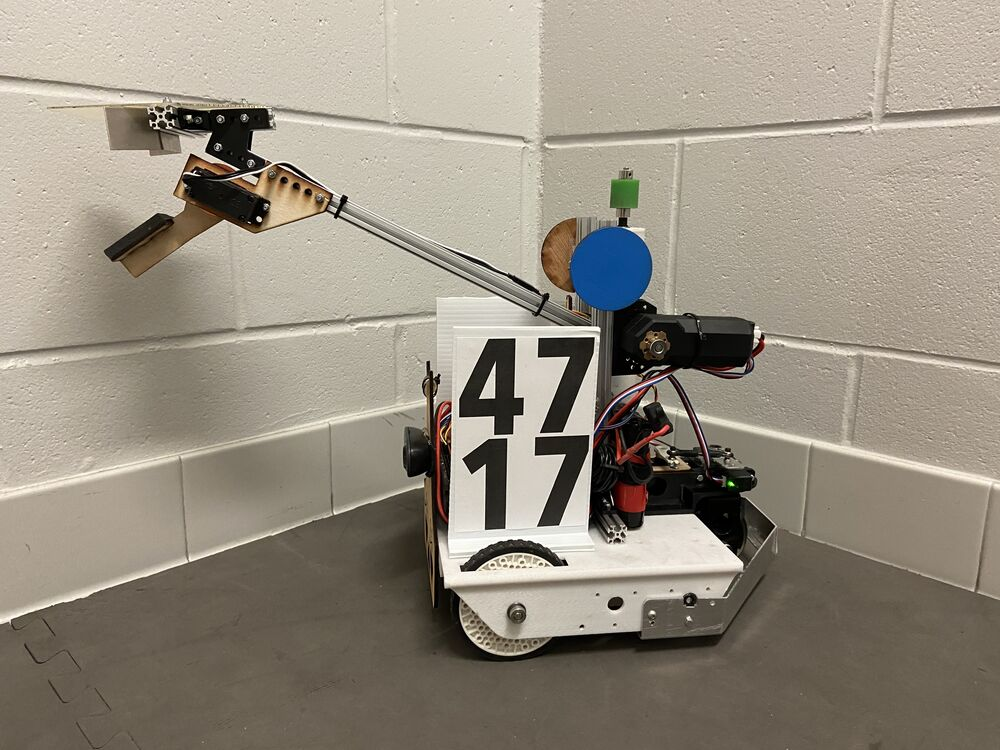
\includegraphics[width=0.95\textwidth]{Meetings/November/11-06-21/11-6-21_Hardware_Figure1 - Nathan Forrer.JPG}
  \caption{The new plastic sides on the drivetrain}
  \label{fig:pic1}
\end{minipage}%
\hfill%
\begin{minipage}[b]{.48\textwidth}
  \centering
  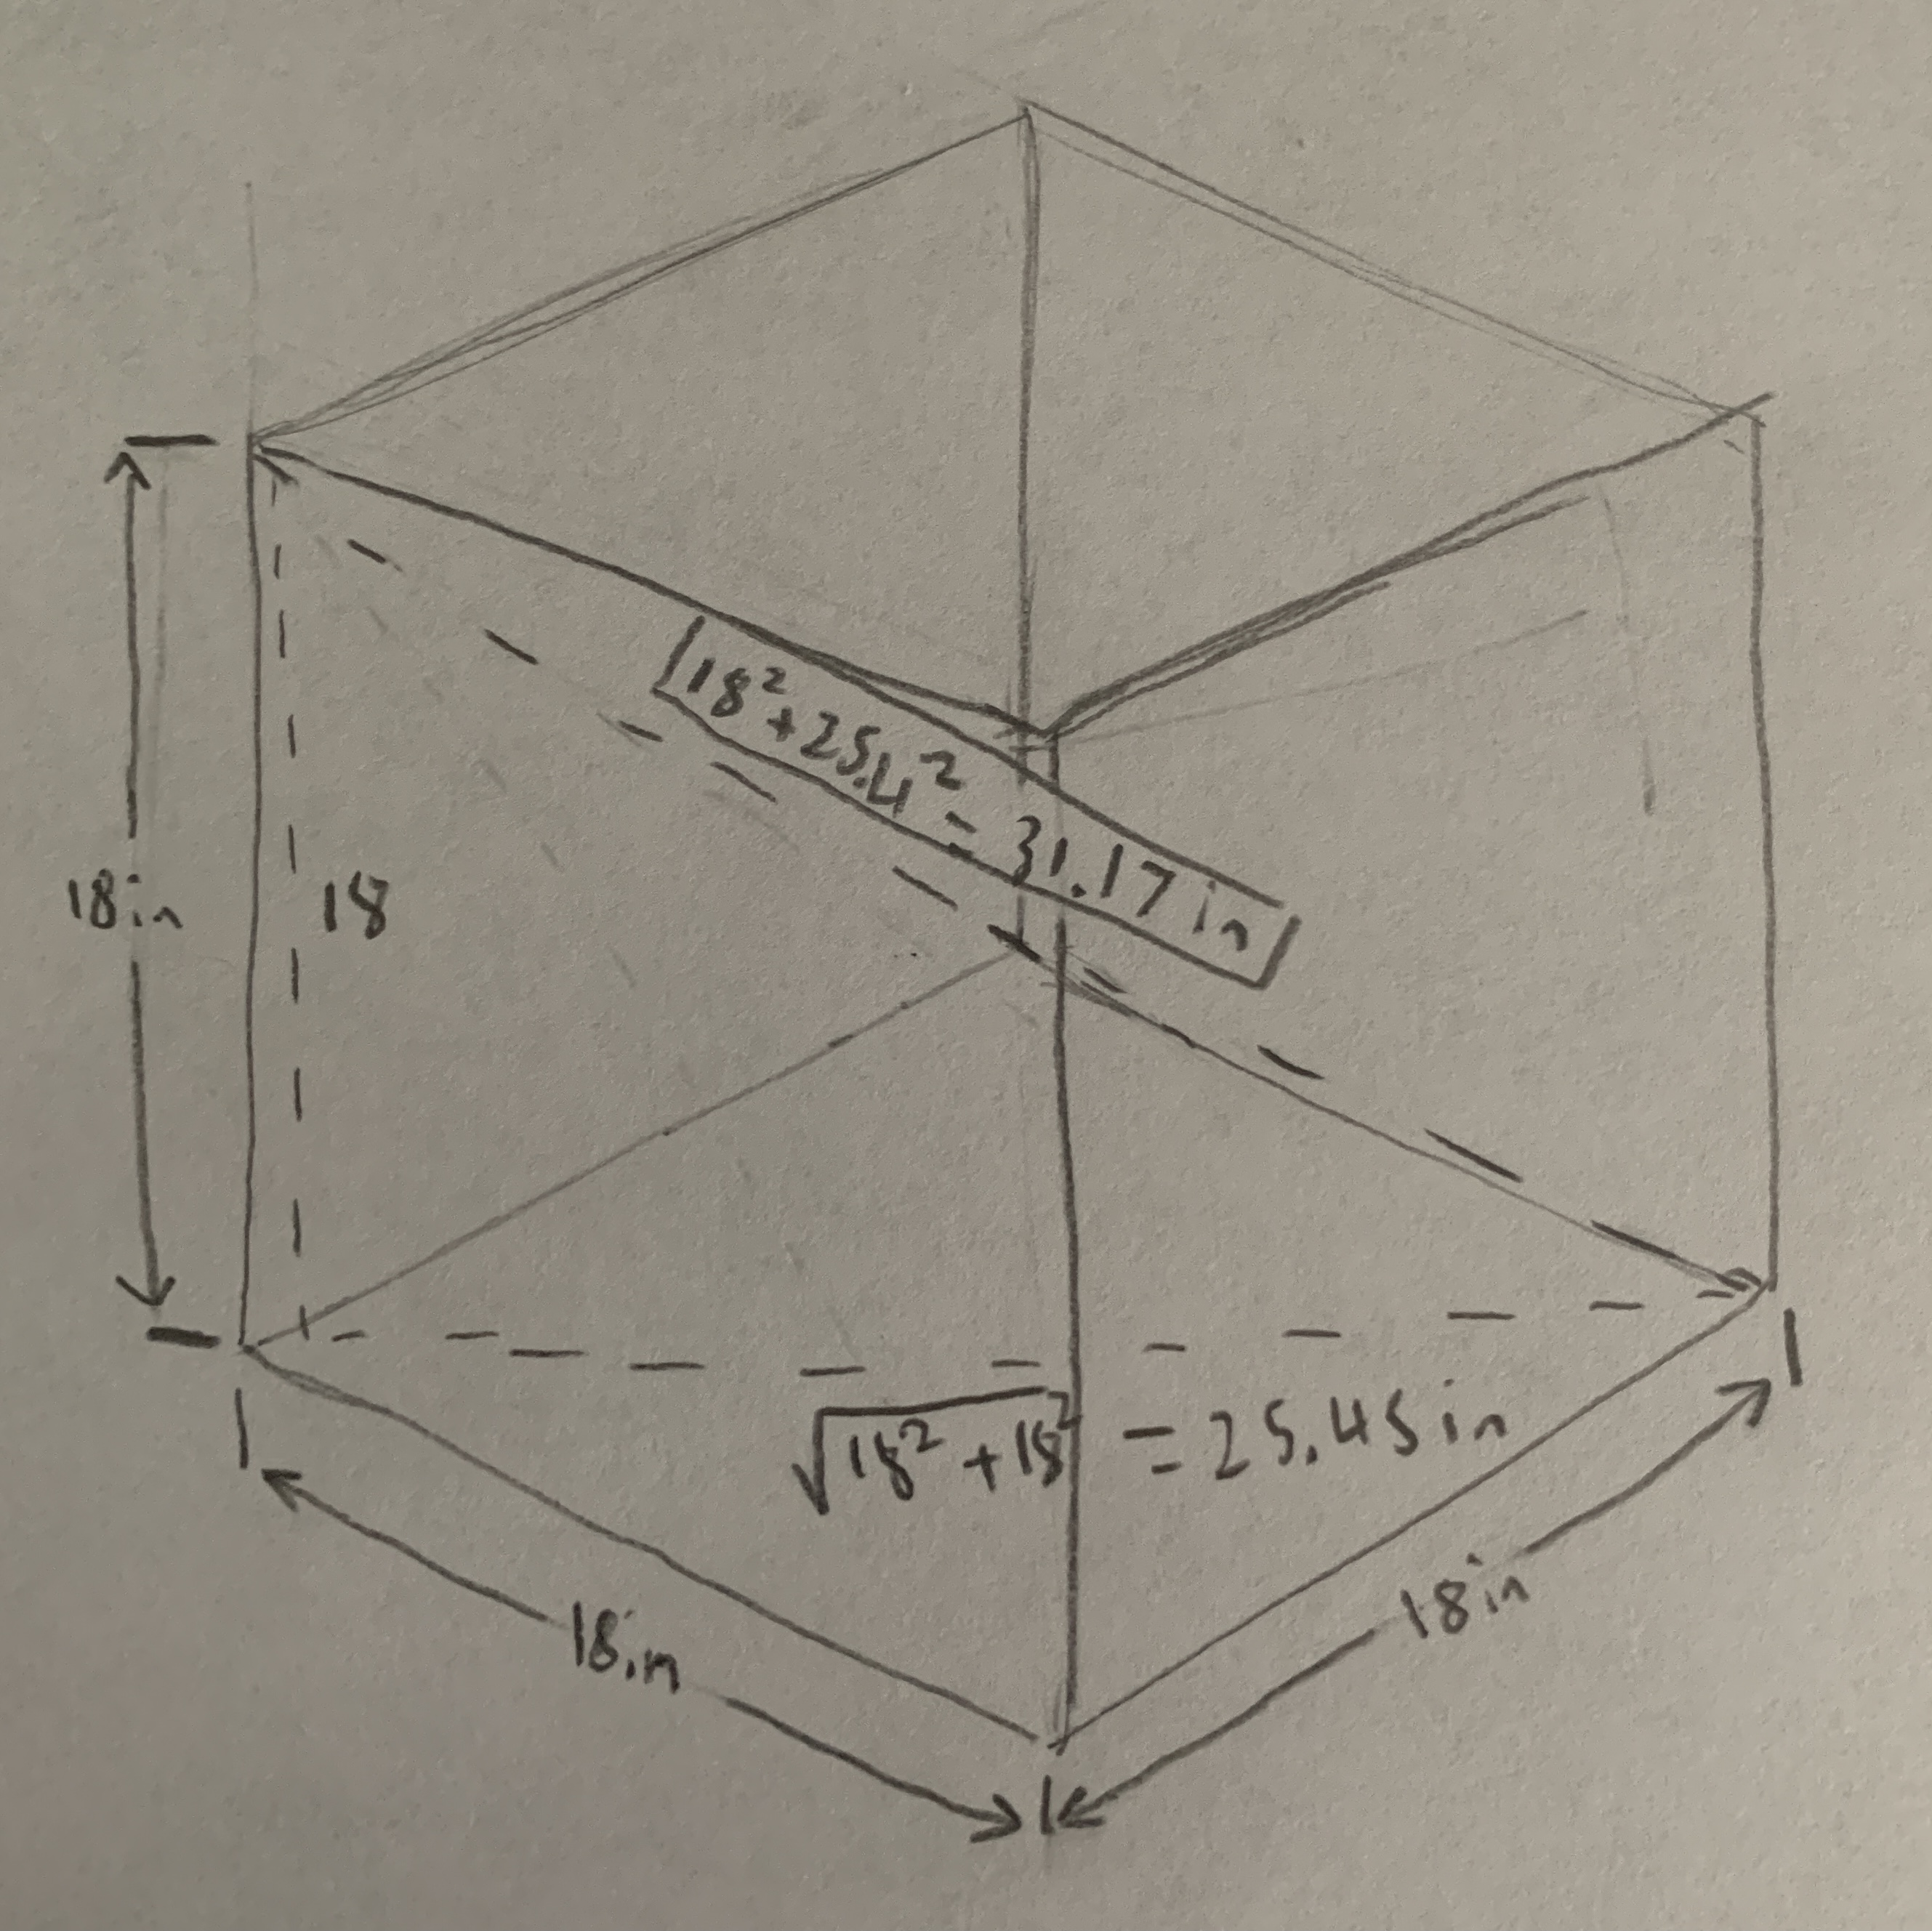
\includegraphics[width=0.95\textwidth]{Meetings/November/11-06-21/11-6-21_Hardware_Figure2 - Nathan Forrer.JPG}
  \caption{Calculating the max cross distance}
  \label{fig:pic2}
\end{minipage}
\end{figure}

\begin{figure}[ht]
\centering
\begin{minipage}[b]{.48\textwidth}
  \centering
  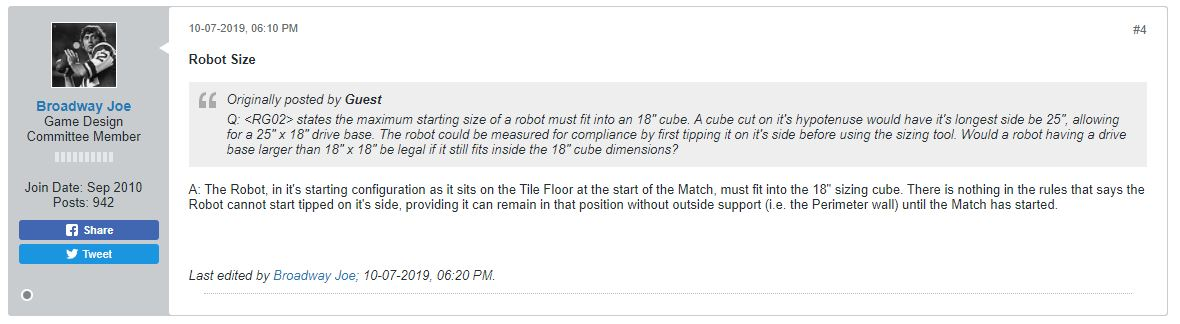
\includegraphics[width=0.95\textwidth]{Meetings/November/11-06-21/11-6-21_Hardware_Figure3 - Nathan Forrer.JPG}
  \caption{Answer from the FTC forums clearing up our question on legality}
  \label{fig:pic3}
\end{minipage}%
\hfill%
\begin{minipage}[b]{.48\textwidth}
  \centering
  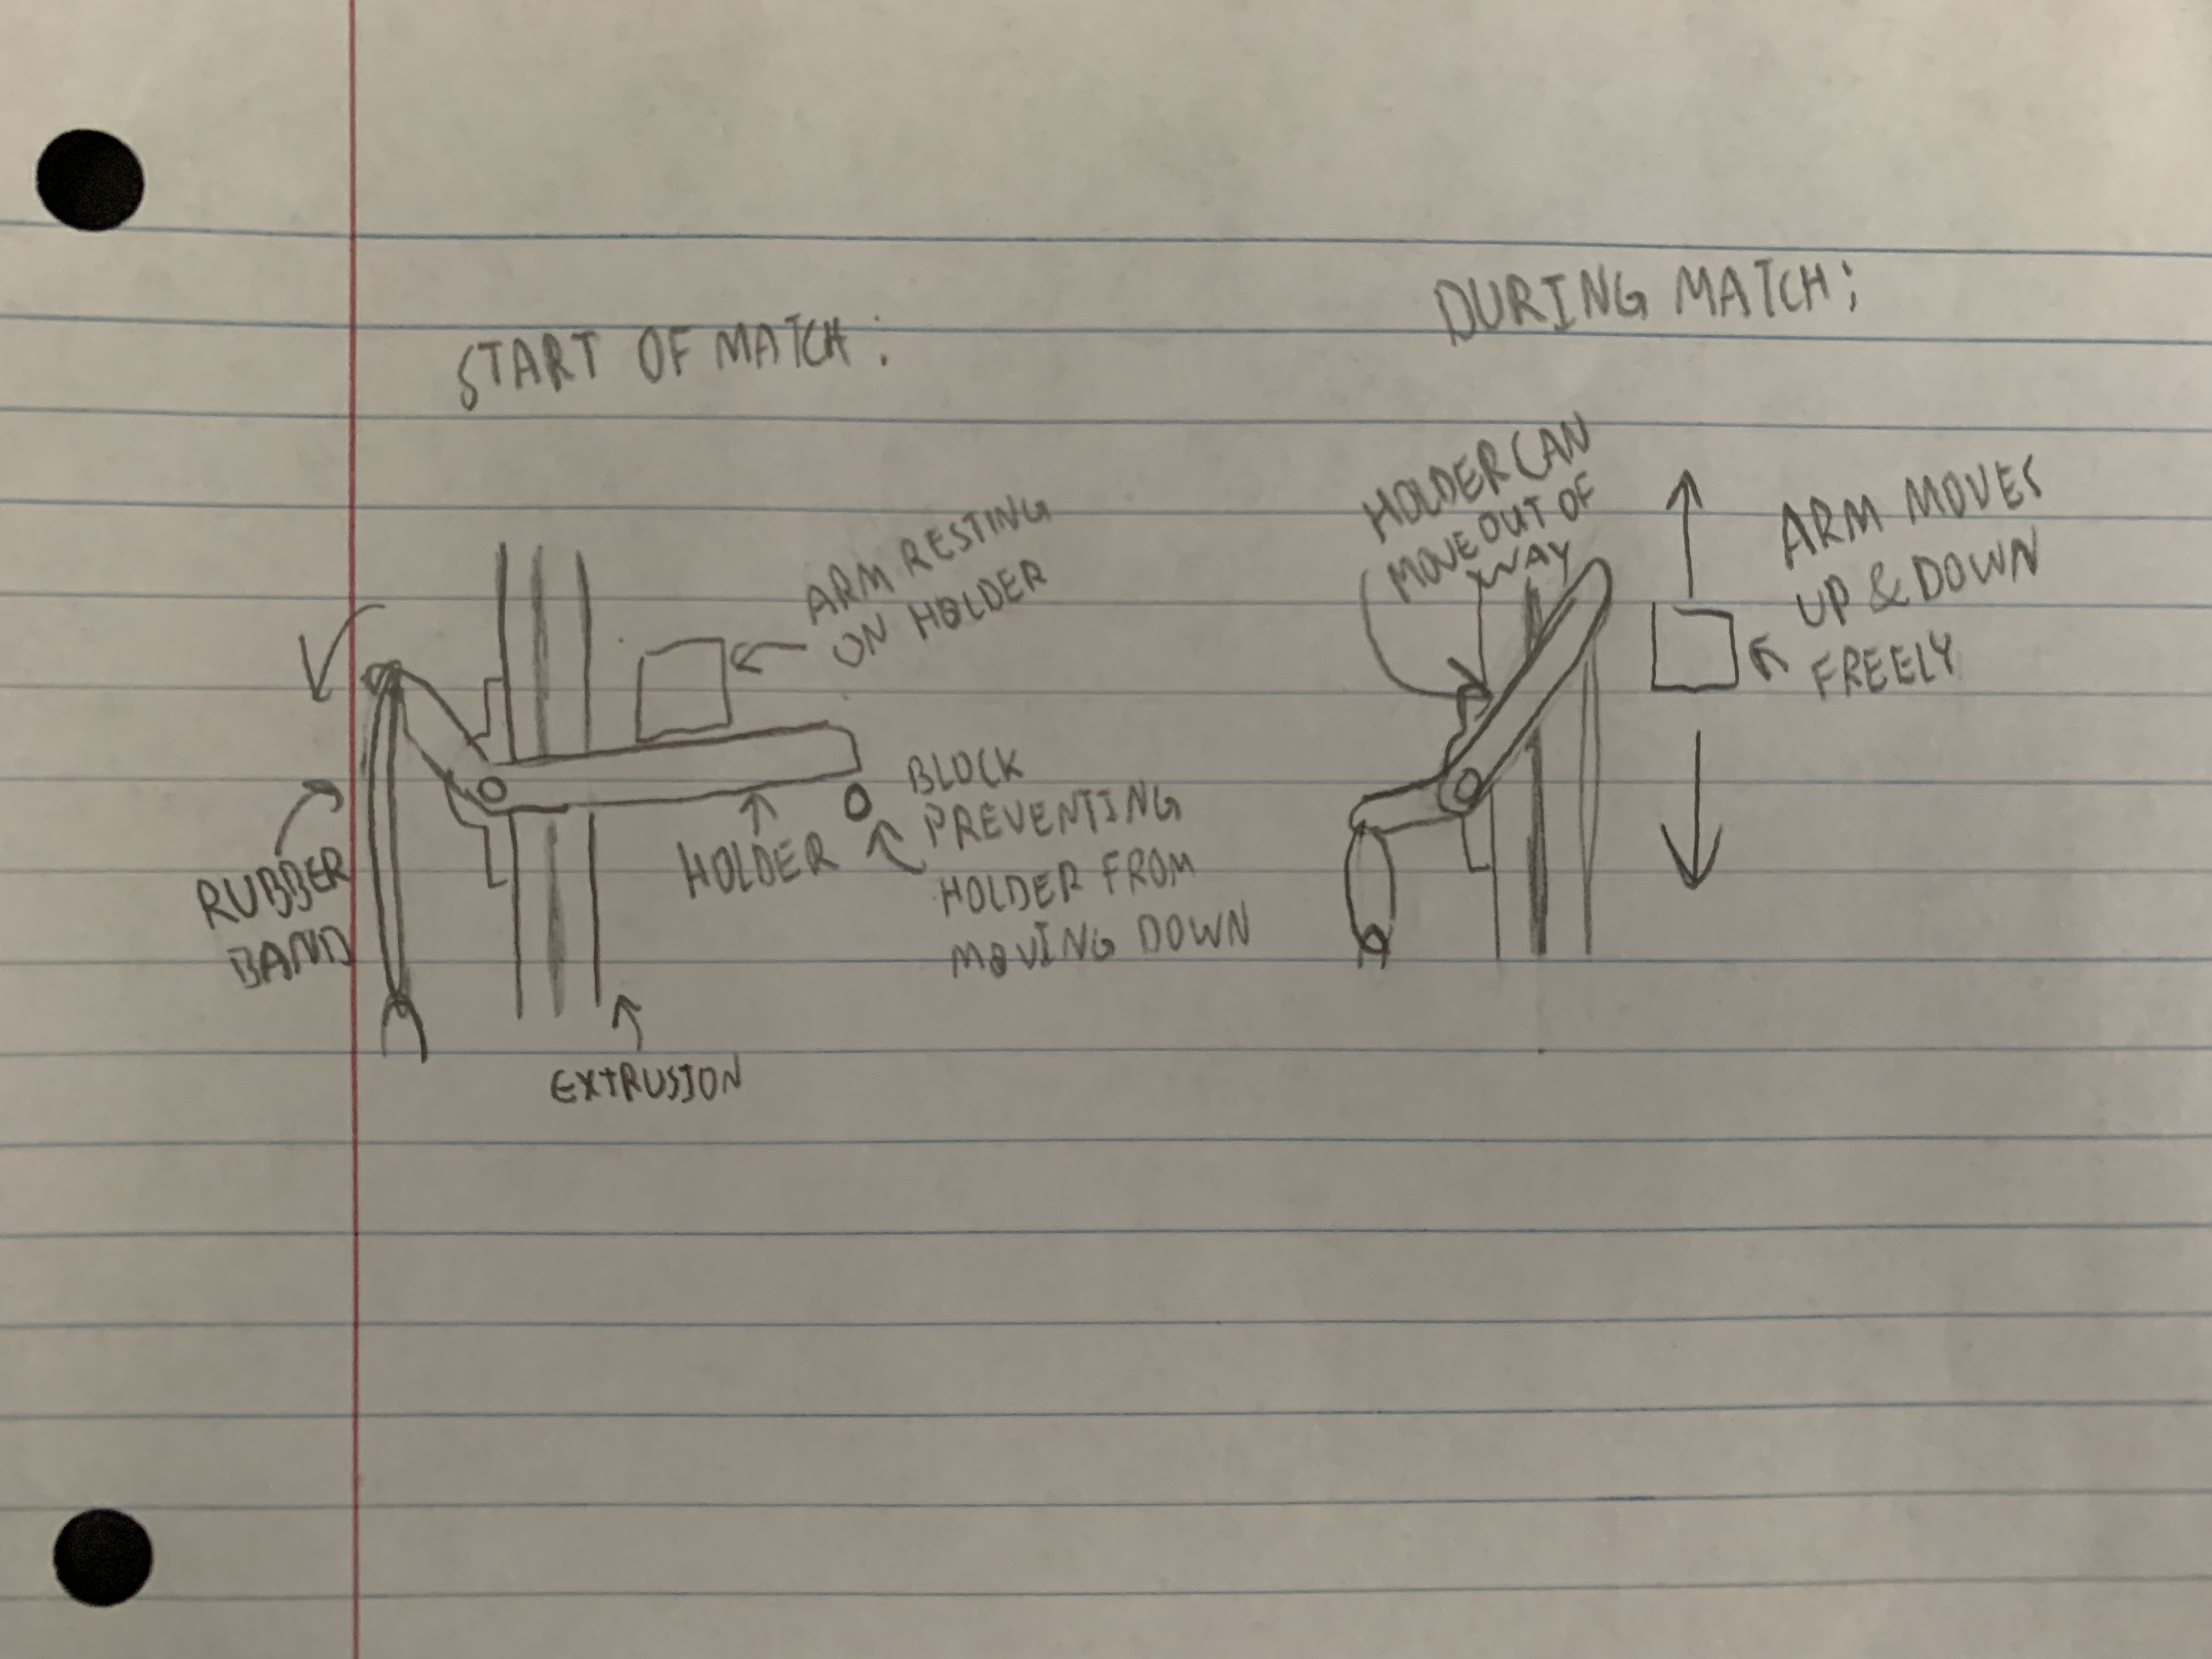
\includegraphics[width=0.95\textwidth]{Meetings/November/11-06-21/11-6-21_Hardware_Figure4 - Nathan Forrer.JPG}
  \caption{Sketches of the holder}
  \label{fig:pic4}
\end{minipage}
\end{figure}


\whatsnext{
\begin{itemize}
    \item CAD and build arm holder to fit robot within 18 inches
\end{itemize} 
}

